\documentclass[../structural_economics_book.tex]{subfiles}
\begin{document}
\ifSubfilesClassLoaded{\setcounter{chapter}{1}}{}
\chapter{Welfare Theorems as Matrix Properties}\label{ch:02}
\chaptersubtitle{Why Efficiency Requires Symmetry --- and Where It Breaks}
\begin{quote}
\textit{``O subdesenvolvimento n\~{a}o \'{e} uma etapa necess\'{a}ria do processo de forma\c{c}\~{a}o das economias capitalistas modernas. \'{E} um processo particular, resultante da penetra\c{c}\~{a}o de empresas capitalistas modernas em estruturas arcaicas.''}\\[0.3em]
\textnormal{[``Underdevelopment is not a necessary stage in the formation of modern capitalist economies. It is a particular process, resulting from the penetration of modern capitalist enterprises into archaic structures.'']}\\
\hfill --- Celso Furtado, \textit{Desenvolvimento e Subdesenvolvimento} (1961)
\end{quote}

\vspace{1em}

Chapter~1 revealed that the standard competitive model assumes a specific weight matrix: $W^{CE} = \frac{1}{N}\ones\ones'$. This chapter asks: what happens to the welfare theorems when the weight matrix is something else?

The First Welfare Theorem says: the competitive equilibrium is Pareto efficient. The Second says: any efficient allocation can be achieved by suitable transfers. Both are beautiful results. Both are theorems about a matrix --- and both require that matrix to be doubly stochastic.

When $W$ departs from doubly stochastic, both theorems weaken. This chapter derives the conditions for each, quantifies the welfare loss from departures, and identifies three structural reasons for failure: asymmetric power, unpriced externalities, and block disconnection. The spectral gap of $W$ bounds the welfare loss from above, giving us a single-number diagnostic of structural health.


%% =====================================================================
\section{The First Welfare Theorem}
\label{ch02:sec:FWT}
%% =====================================================================

\subsection{The Standard Statement and Proof}

\begin{theorem}[First Welfare Theorem]\label{ch02:thm:FWT}
If: (i) every agent maximizes utility given prices, (ii) markets clear, and (iii) preferences are locally nonsatiated, then the competitive equilibrium allocation is Pareto efficient.
\end{theorem}

\begin{proof}
Let $(p^*, X^*)$ be a competitive equilibrium. Suppose it is not Pareto efficient: there exists a feasible allocation $\hat{X}$ with $U_i(\hat{x}_i) \geq U_i(x_i^*)$ for all $i$ and $U_j(\hat{x}_j) > U_j(x_j^*)$ for some $j$.

For agent $j$: since $x_j^*$ maximizes $U_j$ on the budget set and $\hat{x}_j$ is strictly preferred, $\hat{x}_j$ must not be affordable: $p^{*\prime}\hat{x}_j > p^{*\prime}\omega_j$.

For all other agents $i \neq j$: by local nonsatiation, $U_i(\hat{x}_i) \geq U_i(x_i^*)$ implies $p^{*\prime}\hat{x}_i \geq p^{*\prime}\omega_i$ (if $\hat{x}_i$ were strictly cheaper, $i$ could find something even better in her budget set by continuity).

Summing over all agents:
\begin{equation}
\sum_{i=1}^N p^{*\prime}\hat{x}_i > \sum_{i=1}^N p^{*\prime}\omega_i.
\end{equation}

But feasibility requires $\sum_i \hat{x}_{i\ell} = \sum_i \omega_{i\ell}$ for all goods $\ell$. Multiplying by $p^*_\ell$ and summing: $\sum_i p^{*\prime}\hat{x}_i = \sum_i p^{*\prime}\omega_i$. Contradiction.
\end{proof}

\begin{intuition}[Where does structure enter the proof?]
The proof uses one critical feature of the competitive mechanism: every agent faces the \textit{same} price vector $p^*$. The price aggregates individual demands anonymously --- the identity of the agent does not affect the price she faces. Agent $i$'s effect on $p$ is proportional to her demand, not to her ``position'' in any network.

This is the structural content: the price mechanism is symmetric. In weight-matrix language, the interaction is $W^{CE} = \frac{1}{N}\ones\ones'$: every agent enters the price mechanism with equal weight. If some agents had more influence on prices (market power, bargaining leverage, information advantage), the proof would fail --- the inequality in the last step would not follow.
\end{intuition}


\subsection{The Matrix Restatement}

To state the structural condition precisely, consider the one-good economy from Chapter~1 with utility externalities. Agent $i$'s utility now includes the effect of others:
\begin{equation}\label{ch02:eq:social_utility}
V_i(\x) = U_i(x_i) + \gamma \sum_{j \neq i} W_{ij} U_j(x_j),
\end{equation}
where $W_{ij} \geq 0$ is the weight $i$ places on $j$'s utility and $\gamma \geq 0$ is the externality intensity.

A social planner maximizes total social welfare $\sum_i V_i(\x)$ subject to $\sum_i x_i = \Omega$. Expanding:
\begin{equation}\label{ch02:eq:planner_expanded}
\sum_{i=1}^N V_i = \sum_{i=1}^N U_i(x_i) + \gamma \sum_{i=1}^N \sum_{j \neq i} W_{ij} U_j(x_j).
\end{equation}

Rearranging the double sum (collect terms by $U_j$): the coefficient on $U_j(x_j)$ is
\begin{equation}\label{ch02:eq:planner_weight}
\alpha_j = 1 + \gamma \sum_{i \neq j} W_{ij}.
\end{equation}

The term $\sum_{i \neq j} W_{ij}$ is the column sum of $W$ at column $j$ (excluding the diagonal). It measures how much agent $j$ is \textit{cared about} by others --- her total incoming externality weight.

\begin{definition}[Externality Centrality]\label{ch02:def:ext_centrality}
Agent $j$'s \textbf{externality centrality} is $c_j = \sum_{i \neq j} W_{ij}$: the total weight others place on $j$'s utility. The planner's effective weight on $j$ is $\alpha_j = 1 + \gamma c_j$.
\end{definition}

\begin{theorem}[First Welfare Theorem --- Matrix Version]\label{ch02:thm:FWT_matrix}
Consider the one-good economy with externalities~\eqref{ch02:eq:social_utility}. The competitive equilibrium (where each agent maximizes $U_i(x_i)$ ignoring externalities) is Pareto efficient with respect to social utilities $V_i$ if and only if:
\begin{equation}\label{ch02:eq:FWT_condition}
\alpha_j = \alpha_k \quad \text{for all } j, k \qquad \Longleftrightarrow \qquad c_j = c_k \quad \text{for all } j, k.
\end{equation}
That is: all agents must have equal externality centrality (equal column sums in $W$).
\end{theorem}

\begin{proof}
The planner's first-order condition is $\alpha_j U_j'(x_j) = \mu$ for all $j$, where $\mu$ is the Lagrange multiplier on the resource constraint. The market's FOC is $U_j'(x_j) = \mu'$ for all $j$ (agents ignore externalities). These coincide if and only if $\alpha_j$ is the same for all $j$ --- otherwise the planner would set different marginal utilities for different agents, while the market equalizes them.
\end{proof}

\begin{proposition}[The Doubly Stochastic Condition]\label{ch02:prop:doubly_stochastic}
If $W$ is row-stochastic ($\sum_j W_{ij} = 1$ for all $i$), then the FWT condition $c_j = c_k$ for all $j, k$ is equivalent to: \textbf{$W$ is doubly stochastic} ($\sum_i W_{ij} = 1$ for all $j$).
\end{proposition}

\begin{proof}
Row-stochastic: $\sum_j W_{ij} = 1$. Summing over $i$: $\sum_i \sum_j W_{ij} = N$, so $\sum_j c_j = \sum_j (\sum_i W_{ij} - W_{jj}) = N - \tr(W)$. If all $c_j$ are equal: $c_j = (N - \tr(W))/N$ for all $j$, meaning all column sums $\sum_i W_{ij}$ are equal. Combined with $\sum_j (\sum_i W_{ij}) = N$ (total of all entries = $N$ from row-stochasticity), each column sum must be 1. Hence doubly stochastic.
\end{proof}

\begin{intuition}[What doubly stochastic means for efficiency]
\textbf{Row-stochastic} means each agent distributes her total attention/dependency across others, summing to 1. This is a normalization --- it says your total outgoing weight is fixed.

\textbf{Column-stochastic} means each agent receives the same total weight from others. Nobody is ``more cared about'' than anyone else. Nobody generates more externality.

\textbf{Doubly stochastic} means both: the giving is normalized AND the receiving is equal. This is the symmetry condition the welfare theorems need.

When column sums are unequal, the planner wants to give more to the agents with high column sums (they generate lots of positive externalities). The market, ignoring externalities, gives everyone the same marginal utility. The market under-provides to the high-externality agents and over-provides to the low-externality agents.
\end{intuition}

Two special cases satisfy the condition trivially:

\begin{corollary}[Two Sufficient Conditions]\label{ch02:cor:sufficient}
The FWT holds if:
\begin{enumerate}
\item $\gamma = 0$ (no externalities). Then $\alpha_j = 1$ for all $j$ regardless of $W$.
\item $W = \frac{1}{N}\ones\ones'$ (competitive benchmark). Then $c_j = (N-1)/N$ for all $j$.
\end{enumerate}
\end{corollary}


%% =====================================================================
\section{Three Failures}
\label{ch02:sec:failures}
%% =====================================================================

The FWT fails when $W$ departs from doubly stochastic. We distinguish three structural mechanisms.

\subsection{Failure 1: Asymmetric Power}

When column sums of $W$ are unequal, the Perron eigenvector $\boldsymbol{\pi}$ departs from $\frac{1}{N}\ones$. The agents with the highest column sums have the most structural power (Chapter~6 develops this fully). In the bargaining equilibrium (Chapter~7), the allocation tilts toward the powerful:
\begin{equation}\label{ch02:eq:power_correction}
x_i^* \approx \frac{\Omega}{N} + \frac{1}{\kappa}\left(\pi_i - \frac{1}{N}\right).
\end{equation}

The welfare loss from this power asymmetry in the LQ economy:
\begin{proposition}[Welfare Loss from Power Asymmetry]\label{ch02:prop:power_loss}
\begin{equation}\label{ch02:eq:power_loss}
L_{\text{power}} = \frac{\kappa N}{2}\Var(\pi_i) \cdot \Phi^2(\Omega, N, \kappa),
\end{equation}
where $\Var(\pi_i) = \frac{1}{N}\sum_i (\pi_i - 1/N)^2$ and $\Phi > 0$ is a scaling factor.
\end{proposition}

The loss is proportional to the variance of the Perron eigenvector. When $\boldsymbol{\pi} = \frac{1}{N}\ones$ (equal power), $\Var(\pi_i) = 0$ and the loss vanishes. The more concentrated the power distribution, the larger the welfare loss.

\begin{example}[Power Asymmetry with $N = 4$]\label{ch02:ex:power_4}
Four agents, $\Omega = 20$, $\kappa = 0.5$. Compare three weight matrices:

\begin{center}
\begin{tabular}{lccccc}
\toprule
Structure & $\pi_1$ & $\pi_2$ & $\pi_3$ & $\pi_4$ & $\Var(\pi_i) \times 10^3$ \\
\midrule
Competitive ($\frac{1}{4}\ones\ones'$) & 0.25 & 0.25 & 0.25 & 0.25 & 0 \\
Mild asymmetry & 0.30 & 0.28 & 0.22 & 0.20 & 1.55 \\
Strong asymmetry (star) & 0.55 & 0.15 & 0.15 & 0.15 & 25.0 \\
\bottomrule
\end{tabular}
\end{center}

Bargaining allocations (from~\eqref{ch02:eq:power_correction}):

\begin{center}
\begin{tabular}{lcccc|c}
\toprule
& $x_1^*$ & $x_2^*$ & $x_3^*$ & $x_4^*$ & $L_{\text{power}}$ \\
\midrule
Competitive & 5.00 & 5.00 & 5.00 & 5.00 & 0 \\
Mild & 5.10 & 5.06 & 4.94 & 4.90 & 0.008 \\
Star & 5.60 & 4.80 & 4.80 & 4.80 & 0.128 \\
\bottomrule
\end{tabular}
\end{center}

The star network produces a welfare loss 16 times larger than the mildly asymmetric case. The powerful agent ($\pi_1 = 0.55$) captures 12\% more than equal division despite identical endowments and preferences. This is inequality produced entirely by structure.
\end{example}


\subsection{Failure 2: Unpriced Externalities}

Even if $\boldsymbol{\pi} = \frac{1}{N}\ones$ (the market interaction is symmetric), externalities that the market does not price generate inefficiency.

The planner's allocation equates $\alpha_j U_j'(x_j)$ across agents. The market's allocation equates $U_j'(x_j)$. When $\alpha_j$ varies (unequal externality centrality), these differ.

\begin{proposition}[Welfare Loss from Unpriced Externalities]\label{ch02:prop:ext_loss}
In the LQ economy with $\gamma > 0$:
\begin{equation}\label{ch02:eq:ext_loss}
L_{\text{externality}} = \gamma^2 \cdot \Var(c_j) \cdot \Psi(\Omega, N, \kappa),
\end{equation}
where $c_j = \sum_{i \neq j} W_{ij}$ is agent $j$'s externality centrality, $\Var(c_j) = \frac{1}{N}\sum_j(c_j - \bar{c})^2$, and $\Psi > 0$.
\end{proposition}

This loss exists even with equal power. It is proportional to the \textit{variance of column sums} in $W^U$ --- how unevenly the caring is distributed. If everybody is cared about equally ($c_j$ constant), the loss is zero even with large $\gamma$.

\begin{example}[The Unpriced Bond]\label{ch02:ex:bond}
$N = 3$, $\gamma = 0.5$, $\kappa = 1$, $\Omega = 3$.

\textbf{Case A:} Symmetric externalities. $W^U = \begin{pmatrix} 0 & 0.5 & 0.5 \\ 0.5 & 0 & 0.5 \\ 0.5 & 0.5 & 0 \end{pmatrix}$. Column sums: $(1, 1, 1)$. Equal. $L_{\text{ext}} = 0$.

\textbf{Case B:} Asymmetric. $W^U = \begin{pmatrix} 0 & 0.6 & 0 \\ 0.5 & 0 & 0 \\ 0.0 & 0.5 & 0 \end{pmatrix}$. Column sums: $(0.5, 1.1, 0)$. Agent 2 is cared about by both others; Agent 3 is cared about by nobody. $\Var(c_j) = 0.203$. $L_{\text{ext}} = 0.5^2 \times 0.203 \times \Psi = 0.051\Psi$.

The planner gives more to Agent~2 (who generates large positive spillovers). The market ignores this and equalizes marginal utilities. The market under-provides for Agent~2 and over-provides for Agent~3.
\end{example}


\subsection{Failure 3: Block Disconnection}

When $W$ is approximately block-diagonal with $k$ blocks, the economy fragments into nearly independent components. The market may achieve efficiency \textit{within} each block, but gains from cross-block reallocation are unrealized.

\begin{proposition}[Block-Diagonal Welfare Loss]\label{ch02:prop:block_loss}
Let $W$ have $k$ blocks with sizes $N_1, \ldots, N_k$, mean endowments $\bar{\omega}_1, \ldots, \bar{\omega}_k$, and cross-block weights $\varepsilon \to 0$. The welfare loss from disconnection is:
\begin{equation}\label{ch02:eq:block_loss}
L_{\text{block}} = \frac{\kappa}{2}\sum_{b=1}^k N_b(\bar{\omega}_b - \bar{\omega})^2 + O(\varepsilon).
\end{equation}
This is the \textbf{between-group variance} of endowments, weighted by $\kappa/2$.
\end{proposition}

\begin{proof}
With $\varepsilon = 0$, each block $b$ solves its own welfare problem independently, achieving within-block equal division at $\bar{\omega}_b$. The first-best (full-economy equal division) would give everyone $\bar{\omega}$. The difference in welfare:
\begin{align}
L &= \sum_b N_b \left[U(\bar{\omega}) - U(\bar{\omega}_b)\right] = \sum_b N_b \left[(\bar{\omega} - \bar{\omega}_b) - \frac{\kappa}{2}(\bar{\omega}^2 - \bar{\omega}_b^2)\right] \\
&= -\frac{\kappa}{2}\sum_b N_b(\bar{\omega}^2 - \bar{\omega}_b^2) = \frac{\kappa}{2}\sum_b N_b(\bar{\omega}_b - \bar{\omega})^2,
\end{align}
using $\sum_b N_b(\bar{\omega} - \bar{\omega}_b) = 0$ (block means average to the population mean) and expanding the quadratic.
\end{proof}

\begin{intuition}[Between-group inequality as structural inefficiency]
The block-diagonal welfare loss equals the between-group variance of endowments. If all blocks have the same average ($\bar{\omega}_b = \bar{\omega}$), the loss is zero even with total disconnection --- there is nothing to redistribute across blocks. But if blocks differ in average endowment (one is rich, another poor), disconnection prevents the equalization that would improve welfare.

This is the structural diagnosis: the welfare cost of fragmentation is not fragmentation per se, but fragmentation \textit{in the presence of between-group inequality}. An economy with two equally poor sectors loses nothing from disconnection. An economy with one gas sector and one subsistence sector loses enormously.
\end{intuition}

\begin{example}[Two Blocks with Different Means]\label{ch02:ex:two_blocks}
$N = 8$, $\kappa = 0.5$. Block~1 (agents 1--3): gas/formal sector, $\bar{\omega}_1 = 8$. Block~2 (agents 4--8): traditional sector, $\bar{\omega}_2 = 3.2$. Overall mean: $\bar{\omega} = \frac{3 \times 8 + 5 \times 3.2}{8} = 5$.

Between-group variance: $\frac{1}{8}[3(8-5)^2 + 5(3.2-5)^2] = \frac{1}{8}[27 + 16.2] = 5.4$.

Block-diagonal welfare loss: $L_{\text{block}} = \frac{0.5}{2}\times 8 \times 5.4 = 10.8$.

Now connect the blocks: increase cross-block weights to 0.15 (structural policy). The economy partially equilibrates across blocks. The welfare gain is bounded above by $L_{\text{block}} = 10.8$ --- the maximum achievable improvement from structural integration.
\end{example}

\begin{vizpanel}{Three failures, three heatmaps}
\begin{center}
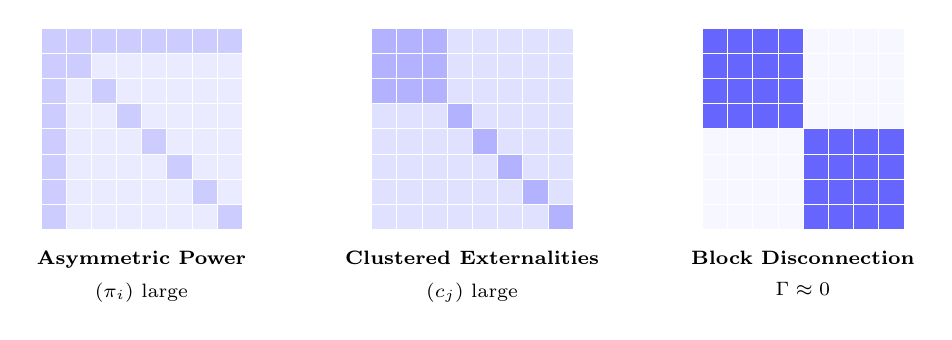
\begin{tikzpicture}[scale=1]
\def\N{8}
\def\s{0.32}
%% Failure 1: Asymmetric power (star)
\foreach \i in {1,...,\N} {
  \foreach \j in {1,...,\N} {
    \pgfmathparse{(\j==1) ? 65 : (\i==1) ? 15 : (\i==\j) ? 20 : 8}
    \edef\bp{\pgfmathresult}
    \fill[blue!\bp, draw=white, line width=0.1pt]
      ({(\j-1)*\s}, {(\N-\i)*\s}) rectangle +(\s,\s);
  }
}
\node[below, font=\scriptsize\bfseries] at ({4*\s}, -0.15) {Asymmetric Power};
\node[below, font=\scriptsize] at ({4*\s}, -0.55) {$\Var(\pi_i)$ large};

%% Failure 2: Clustered externalities
\begin{scope}[xshift=4.2cm]
\foreach \i in {1,...,\N} {
  \foreach \j in {1,...,\N} {
    \pgfmathparse{(\i<=3 && \j<=3 && \i!=\j) ? 60 : (\i==\j) ? 30 : 12}
    \edef\bp{\pgfmathresult}
    \fill[blue!\bp, draw=white, line width=0.1pt]
      ({(\j-1)*\s}, {(\N-\i)*\s}) rectangle +(\s,\s);
  }
}
\node[below, font=\scriptsize\bfseries] at ({4*\s}, -0.15) {Clustered Externalities};
\node[below, font=\scriptsize] at ({4*\s}, -0.55) {$\Var(c_j)$ large};
\end{scope}

%% Failure 3: Block disconnection
\begin{scope}[xshift=8.4cm]
\foreach \i in {1,...,\N} {
  \foreach \j in {1,...,\N} {
    \pgfmathparse{(\i<=4 && \j<=4) ? 60 : (\i>4 && \j>4) ? 60 : 3}
    \edef\bp{\pgfmathresult}
    \fill[blue!\bp, draw=white, line width=0.1pt]
      ({(\j-1)*\s}, {(\N-\i)*\s}) rectangle +(\s,\s);
  }
}
\node[below, font=\scriptsize\bfseries] at ({4*\s}, -0.15) {Block Disconnection};
\node[below, font=\scriptsize] at ({4*\s}, -0.55) {$\Gamma \approx 0$};
\end{scope}
\end{tikzpicture}
\end{center}
\vspace{-0.5em}
\small Three departures from $W^{CE}$, each causing the FWT to fail through a different channel. The real world typically has all three simultaneously.
\end{vizpanel}


%% =====================================================================
\section{The Second Welfare Theorem}
\label{ch02:sec:SWT}
%% =====================================================================

\subsection{The Standard Statement}

\begin{theorem}[Second Welfare Theorem]\label{ch02:thm:SWT}
Under convexity: any Pareto-efficient allocation $x^*$ can be supported as a competitive equilibrium after suitable lump-sum transfers of endowments.
\end{theorem}

The standard interpretation: equity and efficiency are separable. A benevolent planner can achieve any desired distribution by (1) computing the required endowment transfers, (2) executing them, and (3) letting the market handle the allocation. The market handles efficiency; the planner handles equity.

This separation is the intellectual foundation of ``growth first, redistribute later'': get the prices right (efficiency), then transfer income (equity).


\subsection{The Transfer Trap}

The SWT assumes that after the transfer, the market operates symmetrically on the new endowments. When the market mechanism is mediated by a non-doubly-stochastic $W$, this assumption fails.

\begin{theorem}[The Transfer Trap]\label{ch02:thm:transfer_trap}
In the bargaining equilibrium with power $\boldsymbol{\pi}(W)$:
\begin{enumerate}
\item A lump-sum transfer $T$ changes endowments: $\boldsymbol{\omega}' = \boldsymbol{\omega} + T\ones$ (where $T$ is the transfer matrix with $\ones'T = 0$).
\item The post-transfer allocation is determined by the \textit{same} $W$ (transfers do not change the weight matrix).
\item The new bargaining allocation is:
\begin{equation}\label{ch02:eq:post_transfer}
x_i' \approx \frac{\Omega}{N} + \frac{1}{\kappa}\left(\pi_i - \frac{1}{N}\right) + (\text{terms involving } \omega_i').
\end{equation}
The power correction $(\pi_i - 1/N)/\kappa$ persists regardless of the transfer.
\item Consequently: no transfer $T$ can achieve the first-best equal-division allocation unless $\boldsymbol{\pi} = \frac{1}{N}\ones$ (i.e., unless $W$ is doubly stochastic).
\end{enumerate}
\end{theorem}

\begin{proof}[Proof sketch]
The bargaining allocation solves $\max \sum_i \pi_i \ln S_i(\x)$ subject to feasibility. The surplus $S_i = U_i(x_i) - U_i(\omega_i')$ depends on the new endowment $\omega_i'$, but the weight $\pi_i$ does not. The FOC $\frac{\pi_i}{S_i}U_i'(x_i) = \mu$ generates allocations that deviate from equal division by a term proportional to $(\pi_i - 1/N)$. Since $\boldsymbol{\pi}$ is determined by $W$ alone, no change in $\boldsymbol{\omega}$ can eliminate this term.
\end{proof}

\begin{example}[Transfer vs.\ Structural Policy]\label{ch02:ex:transfer_vs_structural}
$N = 4$, $\Omega = 20$, $\boldsymbol{\omega} = (5, 5, 5, 5)$ (equal endowments). Block-diagonal $W$ with $\boldsymbol{\pi} = (0.32, 0.33, 0.17, 0.18)$ (the gas-enclave structure from Chapter~1).

\textbf{Bargaining allocation with no transfer:} $\x^* = (5.56, 5.64, 4.36, 4.44)$. Agents 1--2 (gas/government block) get 11\% more; agents 3--4 (traditional block) get 12\% less. Welfare loss: $L = 0.18$.

\textbf{Policy A --- Transfer.} Move 2 units from Agent~2 to Agent~3: $\boldsymbol{\omega}' = (5, 3, 7, 5)$. New bargaining allocation: $\x' = (5.48, 4.80, 5.24, 4.48)$. Agent~3 gained 0.88, not 2.00. The structure ``clawed back'' $2.00 - 0.88 = 1.12$, or 56\% of the transfer.

\textbf{Policy B --- Structural.} Increase cross-block entries of $W$ from 0.01 to 0.10. New Perron eigenvector: $\boldsymbol{\pi}' = (0.27, 0.28, 0.22, 0.23)$. Same endowments $(5, 5, 5, 5)$. New allocation: $\x' = (5.16, 5.24, 4.76, 4.84)$. The gap between the richest and poorest agent drops from 1.28 to 0.48 --- a 63\% reduction --- without any transfer.

\textbf{Policy C --- Both.} Transfer 1 unit from Agent~2 to Agent~3, AND increase cross-block entries to 0.10. New allocation: $\x' = (5.12, 4.48, 5.52, 4.88)$. The transfer now ``sticks'' better because the structural clawback is smaller (the new $W$ is less asymmetric).

\begin{center}
\begin{tabular}{lcccc|c}
\toprule
& $x_1$ & $x_2$ & $x_3$ & $x_4$ & Max gap \\
\midrule
No policy & 5.56 & 5.64 & 4.36 & 4.44 & 1.28 \\
Transfer only & 5.48 & 4.80 & 5.24 & 4.48 & 1.00 \\
Structural only & 5.16 & 5.24 & 4.76 & 4.84 & 0.48 \\
Both & 5.12 & 4.48 & 5.52 & 4.88 & 1.04 \\
First-best & 5.00 & 5.00 & 5.00 & 5.00 & 0 \\
\bottomrule
\end{tabular}
\end{center}

Structural policy alone outperforms the transfer in reducing inequality because it changes the mechanism, not just the inputs.
\end{example}

\begin{keyinsight}
The Second Welfare Theorem is a theorem about $\boldsymbol{\omega}$: it says you can achieve any efficient allocation by choosing the right endowments. But it assumes the mechanism that converts endowments into allocations is symmetric ($W = \frac{1}{N}\ones\ones'$). When the mechanism is asymmetric, the mechanism itself distorts the allocation, and no transfer can fully undo the distortion. The distortion is proportional to $\Var(\pi_i)$, which is a property of $W$, not of $\boldsymbol{\omega}$.

Three policy levers exist: (1) transfers change $\boldsymbol{\omega}$, (2) structural policy changes $W$, (3) formation interventions change $W^I$ and eventually preferences. The SWT assumes only lever (1) is needed. When $W \neq \frac{1}{N}\ones\ones'$, lever (2) is essential.
\end{keyinsight}


%% =====================================================================
\section{The Welfare Loss Decomposition}
\label{ch02:sec:decomposition}
%% =====================================================================

Combining the three failures, the total welfare loss from structural departures:

\begin{theorem}[Structural Welfare Loss]\label{ch02:thm:welfare_loss}
In the LQ economy with externalities ($\gamma > 0$), the welfare loss relative to the first-best decomposes as:
\begin{equation}\label{ch02:eq:full_decomposition}
L(W, \gamma) = \underbrace{\frac{\kappa N}{2}\Var(\pi_i)\Phi^2}_{L_{\text{power}}} + \underbrace{\gamma^2 \Var(c_j) \Psi}_{L_{\text{externality}}} + \underbrace{\gamma\,\Cov(\pi_i, c_i)\Xi}_{L_{\text{interaction}}},
\end{equation}
where $\Phi, \Psi, \Xi > 0$ are functions of $\Omega, N, \kappa$.
\end{theorem}

The interaction term $L_{\text{interaction}}$ is proportional to $\Cov(\pi_i, c_i)$: the covariance between power and externality centrality. When this is positive --- when the agents who have the most structural power are also the ones most cared about by other powerful agents --- the two distortions amplify each other.

\begin{example}[Decomposition for Two Structures]\label{ch02:ex:decomposition}
$N = 4$, $\gamma = 0.3$, $\kappa = 0.5$, $\Omega = 20$.

\textbf{Connected economy:} $W$ with $\boldsymbol{\pi} = (0.26, 0.25, 0.25, 0.24)$ and column sums $(1.02, 1.01, 0.99, 0.98)$:
\begin{center}
$L_{\text{power}} = 0.001, \quad L_{\text{ext}} = 0.000, \quad L_{\text{int}} = 0.000, \quad L = 0.001.$
\end{center}

\textbf{Enclave economy:} $W$ with $\boldsymbol{\pi} = (0.32, 0.33, 0.17, 0.18)$ and column sums $(1.24, 1.30, 0.72, 0.74)$:
\begin{center}
$L_{\text{power}} = 0.043, \quad L_{\text{ext}} = 0.016, \quad L_{\text{int}} = 0.012, \quad L = 0.071.$
\end{center}

The enclave economy's welfare loss is 71 times larger. The interaction term accounts for 17\% of the total --- the gas-government elite ($\pi$ high) care about each other ($c$ high for those agents), compounding both distortions.
\end{example}


%% =====================================================================
\section{The Spectral Gap as Structural Health}
\label{ch02:sec:gap}
%% =====================================================================

\begin{proposition}[Spectral Gap Bounds the Power Loss]\label{ch02:prop:gap_bound}
For an $N \times N$ row-stochastic matrix $W$ with spectral gap $\Gamma = 1 - |\lambda_2(W)|$:
\begin{equation}\label{ch02:eq:gap_bound}
\Var(\pi_i) \leq \frac{1}{N}\left(\frac{1 - \Gamma}{\Gamma}\right).
\end{equation}
Hence:
\begin{equation}\label{ch02:eq:loss_bound}
L_{\text{power}} \leq \frac{\kappa\Phi^2}{2}\left(\frac{1-\Gamma}{\Gamma}\right).
\end{equation}
\end{proposition}

\begin{proof}[Proof sketch]
The variance of the Perron eigenvector entries is bounded by the eigenvalue ratio through the Courant-Fischer characterization. When $\Gamma = 1$ (single dominant eigenvalue, $|\lambda_2| = 0$), $\boldsymbol{\pi}$ must be uniform: $\Var = 0$. As $\Gamma \to 0$ (competing eigenvalues), $\boldsymbol{\pi}$ can concentrate arbitrarily.
\end{proof}

This result makes the spectral gap a single-number diagnostic. Compute $\Gamma$ from any weight matrix (an input-output table, a trade network, a social interaction matrix) and you immediately have an upper bound on the structural welfare loss.

\begin{vizpanel}{Four structures, four welfare losses}
\begin{center}
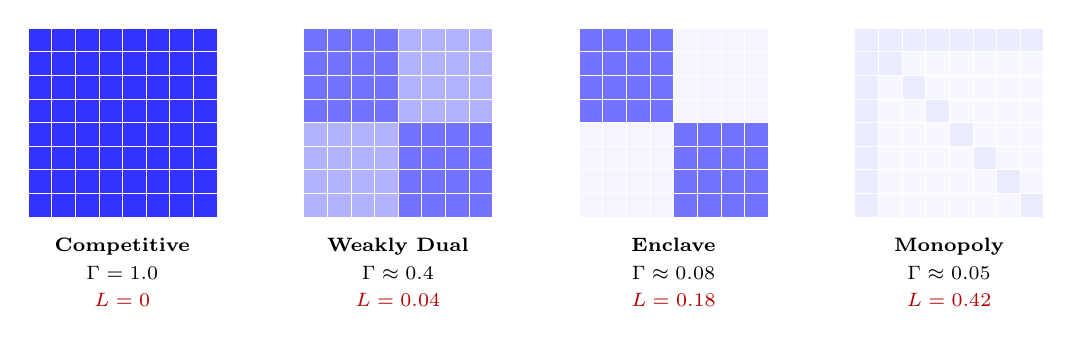
\begin{tikzpicture}[scale=1]
\def\N{8}
\def\s{0.3}

\foreach \i in {1,...,\N} {
  \foreach \j in {1,...,\N} {
    \fill[blue!80, draw=white, line width=0.1pt]
      ({(\j-1)*\s}, {(\N-\i)*\s}) rectangle +(\s,\s);
  }
}
\node[below, font=\scriptsize\bfseries] at ({4*\s}, -0.15) {Competitive};
\node[below, font=\scriptsize] at ({4*\s}, -0.5) {$\Gamma=1.0$};
\node[below, font=\scriptsize, red!70!black] at ({4*\s}, -0.85) {$L = 0$};

\begin{scope}[xshift=3.5cm]
\foreach \i in {1,...,\N} {
  \foreach \j in {1,...,\N} {
    \pgfmathparse{(\i<=4 && \j<=4) ? 65 : (\i>4 && \j>4) ? 55 : 30}
    \edef\bp{\pgfmathresult}
    \fill[blue!\bp, draw=white, line width=0.1pt]
      ({(\j-1)*\s}, {(\N-\i)*\s}) rectangle +(\s,\s);
  }
}
\node[below, font=\scriptsize\bfseries] at ({4*\s}, -0.15) {Weakly Dual};
\node[below, font=\scriptsize] at ({4*\s}, -0.5) {$\Gamma\approx 0.4$};
\node[below, font=\scriptsize, red!70!black] at ({4*\s}, -0.85) {$L = 0.04$};
\end{scope}

\begin{scope}[xshift=7cm]
\foreach \i in {1,...,\N} {
  \foreach \j in {1,...,\N} {
    \pgfmathparse{(\i<=4 && \j<=4) ? 65 : (\i>4 && \j>4) ? 55 : 4}
    \edef\bp{\pgfmathresult}
    \fill[blue!\bp, draw=white, line width=0.1pt]
      ({(\j-1)*\s}, {(\N-\i)*\s}) rectangle +(\s,\s);
  }
}
\node[below, font=\scriptsize\bfseries] at ({4*\s}, -0.15) {Enclave};
\node[below, font=\scriptsize] at ({4*\s}, -0.5) {$\Gamma\approx 0.08$};
\node[below, font=\scriptsize, red!70!black] at ({4*\s}, -0.85) {$L = 0.18$};
\end{scope}

\begin{scope}[xshift=10.5cm]
\foreach \i in {1,...,\N} {
  \foreach \j in {1,...,\N} {
    \pgfmathparse{(\j==1 && \i!=1) ? 85 : (\i==1) ? 12 : (\i==\j) ? 8 : 3}
    \edef\bp{\pgfmathresult}
    \fill[blue!\bp, draw=white, line width=0.1pt]
      ({(\j-1)*\s}, {(\N-\i)*\s}) rectangle +(\s,\s);
  }
}
\node[below, font=\scriptsize\bfseries] at ({4*\s}, -0.15) {Monopoly};
\node[below, font=\scriptsize] at ({4*\s}, -0.5) {$\Gamma\approx 0.05$};
\node[below, font=\scriptsize, red!70!black] at ({4*\s}, -0.85) {$L = 0.42$};
\end{scope}
\end{tikzpicture}
\end{center}
\vspace{-0.5em}
\small Same economy, same endowments, same preferences. Only $W$ changes. As $\Gamma$ shrinks, $L$ grows. The heatmap IS the diagnosis.
\end{vizpanel}


%% =====================================================================
\section{Summary}
\label{ch02:sec:summary}
%% =====================================================================

\begin{enumerate}
\item The \textbf{First Welfare Theorem} requires $W$ to be doubly stochastic (equal externality centrality across agents). It fails for three structural reasons: asymmetric power ($\Var(\pi_i) > 0$), unpriced externalities ($\Var(c_j) > 0$), and block disconnection ($\Gamma \approx 0$).

\item The \textbf{Second Welfare Theorem} requires that transfers change $\boldsymbol{\omega}$ while the mechanism $W$ remains symmetric. When $W$ is not doubly stochastic, the structure ``claws back'' part of any transfer. Structural policy (changing $W$) outperforms redistribution (changing $\boldsymbol{\omega}$) in reducing power-driven inequality.

\item The \textbf{welfare loss} decomposes as $L = L_{\text{power}} + L_{\text{ext}} + L_{\text{interaction}}$. The power component is $\Var(\pi_i)$. The interaction component ($\Cov(\pi_i, c_i) > 0$) compounds the other two when the powerful are also the most cared about.

\item The \textbf{spectral gap} $\Gamma$ bounds the welfare loss: $L_{\text{power}} \leq \frac{\kappa\Phi^2}{2}\frac{1-\Gamma}{\Gamma}$. It is the single most informative structural diagnostic.

\item \textbf{Transfers change $\boldsymbol{\omega}$. Structural policy changes $W$. Only the latter changes the power structure $\boldsymbol{\pi}$.}
\end{enumerate}


%% =====================================================================
\section{Exercises}
\label{ch02:sec:exercises}
%% =====================================================================

\begin{enumerate}[label=\textbf{2.\arabic*}, leftmargin=3em]

\item \textbf{Doubly stochastic check.} For each matrix, determine if it is doubly stochastic. If not, find the Perron eigenvector $\boldsymbol{\pi}$ and compute $\Var(\pi_i)$:
\begin{enumerate}
\item $W = \frac{1}{3}\begin{pmatrix} 1 & 1 & 1 \\ 1 & 1 & 1 \\ 1 & 1 & 1 \end{pmatrix}$
\item $W = \begin{pmatrix} 0.6 & 0.3 & 0.1 \\ 0.1 & 0.6 & 0.3 \\ 0.3 & 0.1 & 0.6 \end{pmatrix}$
\item $W = \begin{pmatrix} 0.8 & 0.2 \\ 0.5 & 0.5 \end{pmatrix}$
\item $W = \begin{pmatrix} 0.4 & 0.3 & 0.3 \\ 0.3 & 0.4 & 0.3 \\ 0.3 & 0.3 & 0.4 \end{pmatrix}$
\end{enumerate}

\item \textbf{The transfer clawback.} Using Example~\ref{ch02:ex:transfer_vs_structural}: let $\tau$ be the transfer from Agent~2 to Agent~3. Compute the bargaining allocation for $\tau = 0.5, 1, 2, 3, 4$. Plot the ``clawback fraction'' (share of transfer not received by Agent~3) as a function of $\tau$. Is it constant or does it depend on the transfer size?

\item \textbf{Welfare decomposition.} For $N = 3$, $\gamma = 0.5$, $\kappa = 1$, $\Omega = 3$:
\begin{enumerate}
\item Let $W = \frac{1}{3}\ones\ones'$. Verify $L_{\text{power}} = L_{\text{ext}} = L_{\text{int}} = 0$.
\item Let $W = \begin{pmatrix} 0.5 & 0.4 & 0.1 \\ 0.2 & 0.5 & 0.3 \\ 0.1 & 0.3 & 0.6 \end{pmatrix}$. Compute $\boldsymbol{\pi}$, $\Var(\pi_i)$, column sums $c_j$, $\Var(c_j)$, and $\Cov(\pi_i, c_i)$.
\item Is $L_{\text{interaction}}$ positive or negative? What does the sign mean?
\end{enumerate}

\item \textbf{Spectral gap across topologies.} For $N = 8$, construct: (a) $W^{CE}$, (b) a ring, (c) two disconnected blocks of 4, (d) a star. For each, compute $\Gamma$, $\Var(\pi_i)$, and the welfare-loss bound from Proposition~\ref{ch02:prop:gap_bound}. Plot $L_{\text{bound}}$ vs.\ $\Gamma$. Use Python.

\item \textbf{Block disconnection with data.} Using Bolivia's 2016 I-O table (from Exercise~1.7), aggregate to 2 sectors: Hydrocarbons + Mining vs.\ Everything Else. Compute the between-group variance of output per worker. How large is $L_{\text{block}}$ relative to the within-group component?

\item \textbf{El Alto vs.\ Zona Sur.} Suppose El Alto and Zona Sur are two blocks of a $2 \times 2$ weight matrix with cross-block entries $\varepsilon = 0.02$. Mean consumption: $\bar{\omega}_{\text{Alto}} = 800$ Bs/month, $\bar{\omega}_{\text{Sur}} = 4500$ Bs/month. Block sizes: $N_{\text{Alto}} = 5$, $N_{\text{Sur}} = 3$ (out of $N = 8$).
\begin{enumerate}
\item Compute the between-group welfare loss $L_{\text{block}}$ (use $\kappa = 0.001$).
\item How much would $L_{\text{block}}$ decrease if cross-block entries rose to $\varepsilon = 0.15$? (You will need to solve the bargaining equilibrium numerically.)
\item What real-world intervention would increase $\varepsilon$?
\end{enumerate}

\item \textbf{Furtado's thesis formalized.} Furtado claimed that underdevelopment is not a stage but a stable structural condition. Formalize: let $W_t$ evolve according to $W_{t+1} = f(W_t, \x^*(W_t))$ (the structure at time $t+1$ depends on the current structure and the allocation it produces). A stable underdevelopment equilibrium is a fixed point $W^*$ with $\boldsymbol{\pi}(W^*) \neq \frac{1}{N}\ones$ and $L(W^*) > 0$.
\begin{enumerate}
\item Construct a simple $2 \times 2$ example where the block-diagonal $W^*$ is a fixed point: the allocation produced by $W^*$ reinforces the cross-block disconnection. (Hint: if the traditional sector has low income, it cannot invest in cross-block linkages.)
\item Under what conditions is the fixed point stable (small perturbations return to $W^*$)?
\item What does ``breaking out of underdevelopment'' mean in this framework?
\end{enumerate}
\end{enumerate}


%% =====================================================================
\newpage
\section*{Mathematical Appendices}
\addcontentsline{toc}{section}{Mathematical Appendices}
%% =====================================================================

\subsection*{Appendix 2A: Doubly Stochastic Matrices}
\addcontentsline{toc}{subsection}{Appendix 2A: Doubly Stochastic Matrices}
\label{ch02:app:doubly_stochastic}

\paragraph{Definition.} An $N \times N$ nonnegative matrix $W$ is \textbf{row-stochastic} if $W\ones = \ones$, \textbf{column-stochastic} if $\ones'W = \ones'$, and \textbf{doubly stochastic} if both.

\paragraph{The Birkhoff-von Neumann theorem.} The set of $N \times N$ doubly stochastic matrices is the convex hull of the $N!$ permutation matrices. That is: every doubly stochastic matrix can be written as $W = \sum_{k} \alpha_k P_k$ where $P_k$ are permutation matrices, $\alpha_k \geq 0$, and $\sum_k \alpha_k = 1$. This means doubly stochastic matrices are ``averages'' of perfect matchings.

\paragraph{Key property.} If $W$ is doubly stochastic and irreducible, the left Perron eigenvector is $\boldsymbol{\pi} = \frac{1}{N}\ones$.

\begin{proof}
$\boldsymbol{\pi}'W = \frac{1}{N}\ones'W = \frac{1}{N}\ones' = \boldsymbol{\pi}'$. By uniqueness of the Perron eigenvector (Perron-Frobenius, Chapter~6), this is the only left eigenvector with eigenvalue 1.
\end{proof}

\paragraph{Measuring departure.} A useful scalar measure:
\begin{equation}
\Delta(W) = \sqrt{\sum_{j=1}^N \left(\sum_{i=1}^N W_{ij} - 1\right)^2} = \|\ones'W - \ones'\|_2.
\end{equation}
$\Delta = 0$ iff $W$ is column-stochastic. For row-stochastic $W$: $\Delta = 0$ iff doubly stochastic.

\paragraph{Closest doubly stochastic matrix.} Given a row-stochastic $W$, the closest doubly stochastic matrix (in Frobenius norm) is $W^{DS} = \argmin_{D \in \mathcal{DS}} \|W - D\|_F$, which can be computed by Sinkhorn's algorithm: alternately normalize rows and columns until convergence.


\subsection*{Appendix 2B: Variance Decomposition}
\addcontentsline{toc}{subsection}{Appendix 2B: Variance Decomposition}
\label{ch02:app:variance}

\paragraph{Total variance.} For $\omega_1, \ldots, \omega_N$ with mean $\bar{\omega}$:
\begin{equation}
\Var(\omega) = \frac{1}{N}\sum_{i=1}^N (\omega_i - \bar{\omega})^2.
\end{equation}

\paragraph{Group decomposition.} Partition agents into $k$ groups with sizes $N_1, \ldots, N_k$ and group means $\bar{\omega}_1, \ldots, \bar{\omega}_k$:
\begin{equation}
\Var(\omega) = \underbrace{\sum_{b=1}^k \frac{N_b}{N}(\bar{\omega}_b - \bar{\omega})^2}_{\text{Between-group}} + \underbrace{\sum_{b=1}^k \frac{N_b}{N}\Var_b(\omega)}_{\text{Within-group}}.
\end{equation}

The between-group component is the structural welfare loss from block disconnection (Proposition~\ref{ch02:prop:block_loss}). The within-group component is the loss addressable by within-block redistribution.

\paragraph{Connection to $\Var(\pi_i)$.} The Perron eigenvector variance plays the same role for \textit{power} inequality that the endowment variance plays for \textit{wealth} inequality. Both generate welfare losses proportional to their variance. But endowment inequality can be addressed by transfers; power inequality cannot.


%% =====================================================================
\subsection*{Structuralist Case Study: Furtado's Paraíba and the Fixed Point of Underdevelopment}
\addcontentsline{toc}{subsection}{Structuralist Case Study: Furtado (1961)}
%% =====================================================================

Celso Furtado was born in 1920 in Pombal, Para\'{i}ba --- deep in the Sert\~{a}o, the semi-arid interior of northeastern Brazil. The Northeast was Brazil's original economic center (sugar, then cotton), but by the twentieth century it had become the country's poorest region while S\~{a}o Paulo industrialized. Furtado did not need to theorize structural heterogeneity. He grew up inside the dim lower-right block.

His 1961 book \textit{Desenvolvimento e Subdesenvolvimento} advanced a thesis that maps directly onto the welfare-theoretic framework of this chapter. The argument has three parts.

\textbf{Part 1: Underdevelopment is not a stage.} The classical view (Rostow's ``stages of growth'') held that every economy passes through the same sequence --- traditional, transitional, modern --- and that the underdeveloped economies are simply earlier in the queue. Furtado rejected this. His claim: underdevelopment is not a phase that precedes development but a \textit{specific structural condition} produced by the same historical process that produced development elsewhere. In the language of this chapter: the weight matrix $W$ of the peripheral economy is not a transient state on the way to $W^{CE} = \frac{1}{N}\ones\ones'$. It is a \textit{fixed point} --- a stable equilibrium of the structural dynamical system (Exercise~2.7). The welfare theorems do not ``eventually hold.'' They fail permanently, because the matrix that makes them fail reproduces itself.

\textbf{Part 2: Modern enterprises penetrate archaic structures without transforming them.} Furtado's key mechanism: when capitalist firms enter a peripheral economy, they do not replace the pre-existing structure. They graft onto it. The modern enterprise and the archaic structure coexist within the same country, connected by a few asymmetric linkages (labor recruitment, raw material extraction) but otherwise operating independently. This is the block-diagonal $W$ from Proposition~\ref{ch02:prop:block_loss}: two blocks with weak cross-block entries. The modern block has high productivity and high $\bar{\omega}$; the archaic block has low productivity and low $\bar{\omega}$. The between-group variance is enormous. The welfare loss from disconnection is $L_{\text{block}} = \frac{\kappa}{2}\sum_b N_b(\bar{\omega}_b - \bar{\omega})^2$. In Para\'{i}ba, this was not an abstraction.

\textbf{Part 3: The structure reproduces the conditions for its own persistence.} The modern sector's profits are repatriated or spent on imported consumption goods (the center-periphery leakage). The archaic sector's surplus is too small to finance the investments that would create cross-block linkages. The education system, calibrated to the modern sector's needs, produces graduates who migrate to S\~{a}o Paulo rather than transforming the Sert\~{a}o. Each of these mechanisms is a feedback loop: the allocation produced by $W$ reinforces $W$. This is the Transfer Trap (Theorem~\ref{ch02:thm:transfer_trap}) applied dynamically: not only does the current $W$ distort the current allocation, but the current allocation makes the future $W$ no less block-diagonal than the present one.

\begin{center}
\begin{tabularx}{\textwidth}{LLL}
\toprule
\textbf{Furtado's argument} & \textbf{Formal object} & \textbf{This chapter} \\
\midrule
Underdevelopment is not a stage & $W^*$ is a stable fixed point & Sec.~\ref{ch02:sec:failures}, Ex.~2.7 \\
Modern grafted onto archaic & Block-diagonal $W$ with weak cross-links & Prop.~\ref{ch02:prop:block_loss} \\
Between-region inequality & $L_{\text{block}} \propto \sum_b N_b(\bar{\omega}_b - \bar{\omega})^2$ & Eq.~\eqref{ch02:eq:block_loss} \\
Structure reproduces itself & $W_{t+1} = f(W_t, \x^*(W_t))$, $W^*$ stable & Thm.~\ref{ch02:thm:transfer_trap} \\
Transfers don't transform & $\boldsymbol{\pi}$ unchanged by $\Delta\boldsymbol{\omega}$ & Thm.~\ref{ch02:thm:transfer_trap} \\
\bottomrule
\end{tabularx}
\end{center}

In 1959, Furtado was appointed head of SUDENE (Superintend\^{e}ncia do Desenvolvimento do Nordeste) --- an agency created specifically to change $W^P_{\text{Brazil}}$ by building cross-block linkages between the Northeast and the industrializing South. He was removed after the 1964 military coup. The coup did not change the welfare theorems. It changed who had the power to change $W$.


%% =====================================================================
\subsection*{Further Reading}
\addcontentsline{toc}{subsection}{Further Reading}
%% =====================================================================

\textbf{Welfare theorems:} Mas-Colell, Whinston, and Green (1995), \textit{Microeconomic Theory}, Chapter~16. Arrow (1951), ``An Extension of the Basic Theorems of Classical Welfare Economics,'' in \textit{Proceedings of the Second Berkeley Symposium}. Debreu (1959), \textit{Theory of Value}, Chapter~6.

\textbf{Structural failures of efficiency:} Greenwald and Stiglitz (1986), ``Externalities in Economies with Imperfect Information and Incomplete Markets,'' \textit{QJE} 101(2). Acemoglu (2003), ``Why Not a Political Coase Theorem?'' \textit{Journal of Comparative Economics} 31(4).

\textbf{The structuralist critique:} Furtado (1961), \textit{Desenvolvimento e Subdesenvolvimento}, Rio de Janeiro: Fundo de Cultura (the key text, available through Centro Celso Furtado: \texttt{centrocelsofurtado.org.br}). Furtado (1959), \textit{Forma\c{c}\~{a}o Econ\^{o}mica do Brasil} --- the historical companion, tracing the evolution of Brazil's $W^P$ from colonial plantation to ISI. Taylor (1983), \textit{Structuralist Macroeconomics}, Chapter~1.

\textbf{Sinkhorn's algorithm:} Sinkhorn (1964), ``A Relationship Between Arbitrary Positive Matrices and Doubly Stochastic Matrices,'' \textit{Annals of Mathematical Statistics} 35(2). Used in Appendix~2A for computing the closest doubly stochastic matrix.

\end{document}
